\label{sec:brushing}
The tracking typically contain a few frames where either the view of the particle is visually obstructed or is not detected correctly 
leading to spikes in the data. To make further theoretical analysis possible the data is corrected by removing such points manually. The basis for removal is a large discontinuity in the data, and could largely be eliminated with algorithmic means. However in particular for $n_z$ it is very difficult to write an algorithm that will catch all possible edge cases. For example $n_z$ have peaks that make its derivative non continuous which means that cannot be use as a criterion. It's thus simpler to look at the analysis program and remove the points where the particle cannot be traced accurately due to noise. 

An example of data before and after correction can be seen in figure \ref{fig:brushed} and all uncorrected data files will be available at \url{http://goo.gl/jgzSXe}.

\begin{figure}[H]
\centering
\begin{subfigure}[3a]{0.40\textwidth}
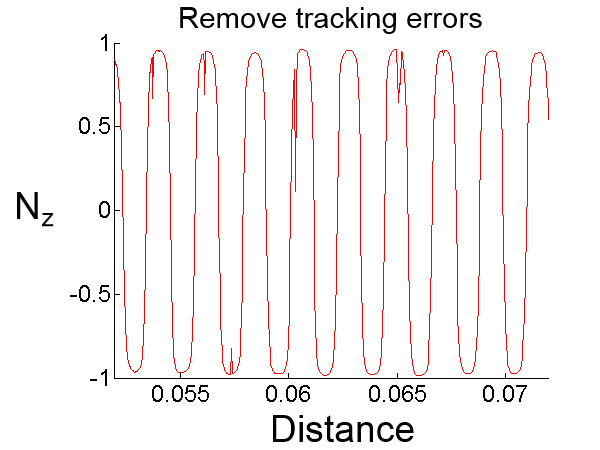
\includegraphics[width=\textwidth]{figures/method/Brushing1.png}
\caption{$n_x$ time series before correction.}\label{fig:prebrush}
\end{subfigure}\hspace{1em}%
\begin{subfigure}[3b]{0.40\textwidth}
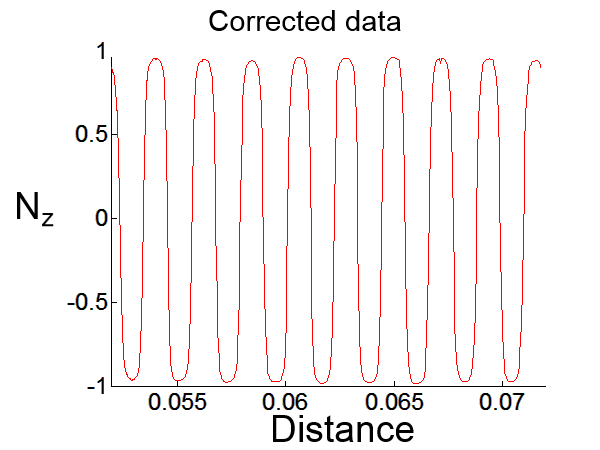
\includegraphics[width=\textwidth]{figures/method/Brushing2.png}
\caption{$n_x$ time series after correction.}\label{fig:postbrush}
\end{subfigure} \\
\caption{Shows a time series of $n_x$ before and after removing points where a significant amount of noise disturbed the tracking. } \label{fig:brushed}
\end{figure}
